\chapter{Fortran90の応用3〜運動方程式の解法〜}

前回の演習では一階の連立微分方程式の数値シミュレーションを取り扱った.  
今回はこれを応用して, 二階の微分方程式である運動方程式の解法を学び, 
スポーツの一場面を力学的に解析してみよう. 

\section{物体の自由落下のシミュレーション}
ここでは, 以下のような質点の自由落下をシミュレートする. 
\begin{figure}[ht]
\centering
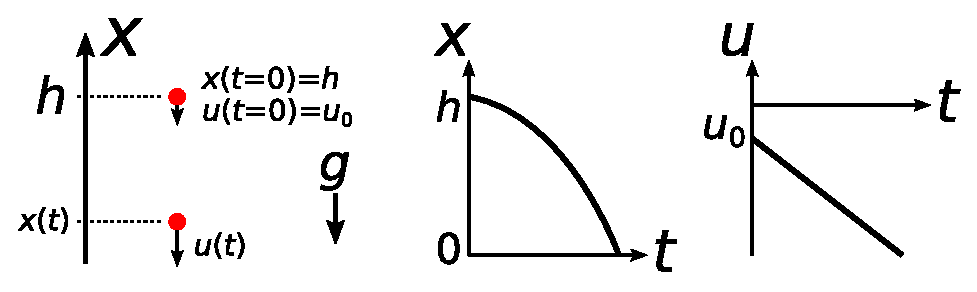
\includegraphics[width=0.8\linewidth]{9_fortran6/figs/freefall.eps}
\caption{自由落下運動の模式図. 時刻$t = 0$ に $x(0)=h$ で鉛直方向に速度$u_0$で
運動している物体(図の赤丸)の軌道をシミュレートする. 
位置$x$および速度$u$の模式図は中・右図のようになる. }
\end{figure}

質点の質量を$m$, 重力加速度を$g$, 初期位置を$h$, 初速を$u_0$とする.
鉛直座標として$x$をとると, 運動方程式は
\begin{equation}
m\frac{d^2x}{dt^2}=-mg, \ \ \ x(0)=h, \ \ \ \frac{dx}{dt}(0)=u_0
\label{eq_freefall}
\end{equation}
で与えられる. 
その解は
\begin{equation}
x(t)=h+u_0t-\frac{1}{2}gt^2.
\end{equation}
であるが, これをコンピュータを用いて近似的に求めてみよう. 

式(\ref{eq_freefall})を以下のように変形することで一階の連立微分方程式が得られる.
\begin{equation}
\frac{dx}{dt}=u, \ \ \ x(0)=h,
\end{equation}
\begin{equation}
\frac{du}{dt}=-g, \ \ \ u(0)=u_0.
\end{equation}
これを前回学習したEuler法を用いて数値的に解けばよい.
プログラムの例を以下に示す.
計算した$x, u$の時間変化をグラフにし, 厳密解と比較してみよ. 

\newpage
\lstinputlisting[caption={質点の自由落下シミュレーション. }, label=freefall]{9_fortran6/codes/FreeFall.f90}

%------------- 空気抵抗下での鉛直落下 ----------------------
\section{空気抵抗下での自由落下のシミュレーション}
上の例では空気抵抗の影響を無視したが, 実際の系では多少なりとも空気抵抗が影響を及ぼす. 
一般に, 空気抵抗は, 物体の速度の大きさの二乗に比例し, その向きと逆方向の力を及ぼす. 
具体的には, 空気抵抗力の大きさ$D$は物体が球形の場合, 
\begin{equation}
D=\frac{1}{2}\rho |\mathbf{u}|^2 \pi a^2 C_D,
\end{equation}
と表せる. 
なお, $|\mathbf{u}|$は速度ベクトル$\mathbf{u}$の絶対値を表す. 
ここで, $\rho$は空気の密度, $a$は球の半径である.
また, 抗力係数$C_D$はある条件\footnote{
Reynolds数$Re=2aU/\nu$ ($\nu$は空気の動粘性係数, $U$は系の代表速度)と呼ばれる無次元数が
$5 \times 10^2 < Re < 1 \times 10^5$のときにこの近似が有効である. 
}
のもとでは約0.44で一定であることが知られている

空気抵抗を考慮した場合, 解くべき微分方程式は, 
\begin{equation}
\frac{dx}{dt}=u, \ \ \ x(0)=h,
\end{equation}
\begin{equation}
\frac{du}{dt}=-g-\frac{D}{m}\frac{u}{|u|}, \ \ \ u(0)=u_0.
\end{equation}
となる. 

空気抵抗の影響を含めた落下運動のシミュレーションを行うソースコードは以下のように書ける. 
計算結果を, 空気抵抗のない場合と比較してみよ. 
\lstinputlisting[caption={空気抵抗下での質点の落下シミュレーション. }, label=freefall]{9_fortran6/codes/FreeFall_friction.f90}

\subsection*{$<$演習課題6.1$>$}
\begin{enumerate}
\item 大きいリンゴと小さいリンゴはどちらが早く落ちるか? リンゴの密度は等しいものとする. 
\item 同じ大きさのリンゴと鉄球はどちらが早く落ちるか?
\item 同じ重さのリンゴと鉄球はどちらが早く落ちるか?
\end{enumerate}

\section{空気抵抗下での野球ボール軌道のシミュレーション}
ここでは, 以下の図に示すような野球ボールの軌道をシミュレートする. 
ここで野球ボールは, 以下のように時刻$t=0$で%原点($x=0, z=0$)から, 
斜め方向に$x, z$方向の速度成分$u_x, u_z$で打ち出される. 

\begin{figure}[ht]
\centering
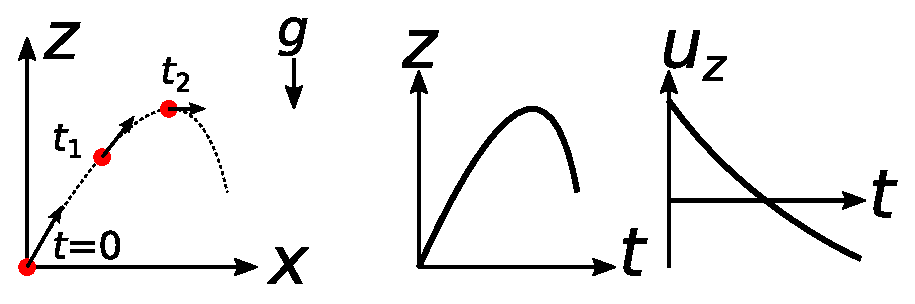
\includegraphics[width=0.8\linewidth]{9_fortran6/figs/shahou.eps}
\caption{野球ボール軌道の模式図. 時刻$t = 0$ に $x(0)=0, z(0)=0$ で
斜め方向に速度$u_x(0), u_z(0)$で打ち出された球状の物体(図の赤丸)が, 
重力および空気抵抗の影響を受けて運動する様子をシミュレートする. 
位置$z$および$z$方向速度$u_z$の模式図は中・右図のようになる. }
\end{figure}

この場合, 空気抵抗の$x, z$方向の成分はそれぞれ
\begin{equation}
  \begin{aligned}
    D_x &= -D u_x / |\mathbf{u}| \\
    D_z &= -D u_z / |\mathbf{u}| \\
  \end{aligned}
\end{equation}
と表される. 

運動方程式は, 速度に関する微分方程式
\begin{equation}
  \begin{aligned}
    \frac{\mathrm{d}u_x}{\mathrm{d}t} &= \frac{D_x}{m},\\
    \frac{\mathrm{d}u_z}{\mathrm{d}t} &= \frac{D_z}{m} - g,\\
  \end{aligned}
\end{equation}
と, 位置に関する微分方程式
\begin{equation}
  \begin{aligned}
    \frac{\mathrm{d}x}{\mathrm{d}t} &= u_x,\\
    \frac{\mathrm{d}z}{\mathrm{d}t} &= u_z,\\
  \end{aligned}
\end{equation}
と表される. 


\if0 %%%%%%%%%%%%%%%%%%%%%%%%%%%%%%%%%%%%%%%%%%%%%%%%%%%%%%%%%%%%%%%
\subsection{Reynolds数が小さい場合}
$Re<0.1$のとき, 抗力係数は理論的に
\begin{equation}
C_D=\frac{24}{Re}
\end{equation}
となることが知られている.

このとき, 運動方程式は
\begin{equation}
m\frac{d^2 x}{dt^2}=-6\pi \rho \nu a \frac{dx}{dt},
\end{equation}
\begin{equation}
m\frac{d^2 y}{dt^2}=-mg-6\pi \rho \nu a \frac{dy}{dt},
\end{equation}
となり, 抵抗は速さの一乗に比例する.
比例係数$6\pi \rho \nu a$は物性値と球の大きさによって決まる.

\begin{table}[h]
\centering
\begin{tabular}{ccc}
\hline
パラメータ & 値 & 備考 \\
\hline
質量$m$ [kg] & - & 適当に与える \\ \hline
半径$a$ [m] & - & 適当に与える \\ \hline
重力加速度$g$ [m/s$^2$] & 9.80665 & - \\ \hline
空気の密度$\rho$[kg/m$^3$] & 1.261 & 280Kの場合 \\
 & 1.176 & 300Kの場合 \\ \hline
空気の動粘性係数$\nu$[m$^2$/s] & 1.395 $\times 10^{-5}$ & 280Kの場合 \\
 & 1.579 $\times 10^{-5}$ & 300Kの場合 \\ \hline
水の密度$\rho$[kg/m$^3$] & 9.999 $\times 10^2$ & 280Kの場合 \\
 & 9.966 $\times 10^2$ & 300Kの場合 \\ \hline
水の動粘性係数$\nu$[m$^2$/s] & 1.436 $\times 10^{-6}$ & 280Kの場合 \\
 & 8.574 $\times 10^{-7}$ & 300Kの場合 \\ \hline
Reynolds数$Re$[-] & $\frac{2aU}{\nu}$ & 計算する \\ \hline
抗力係数$C_D$[-] & $\frac{24}{Re}$ & $Re<0.1$における理論式 \\
& $(\sqrt{\frac{24}{Re}}+0.5407)^2$ & $Re< 6000$における経験式 \\
& $0.44$ & $5 \times 10^2 < Re < 1 \times 10^5$における近似値 \\
& & (この範囲で抵抗は速度の二乗に比例) \\ \hline
スケールハイト$H_\rho$[m] & 8 $\times 10^3$ & 実際は温度によって変化する \\ \hline
\end{tabular}
\end{table}
\fi %%%%%%%%%%%%%%%%%%%%%%%%%%%%%%%%%%%%%%%%%%%%%%%%%%%%%%%%%%%%%%%%

\subsection*{$<$演習課題6.2$>$}
大谷翔平は野球ボールを最大球速 165km/h で投げることができる. 
彼は地面に対しどの方向(角度$\theta$)に対してもこの初速で野球ボールを投げ出すことができ, 
彼の身長は193cmで腕の長さは85cmとする. 
また, ボールの回転は考慮しないものとする. 

これら仮定のもとで, 以下の状況をシミュレート	せよ. 
\begin{enumerate}
% TODO 問題が難しすぎる気がする. 
\item 空気抵抗がない場合($C_D=0$), 適当な角度$\theta$に対するシミュレーションをおこない, 解析解と比較せよ. 
ボールのリリース点の高さは適当に設定すること. 
\item 空気抵抗がある場合のシミュレーションをおこない, 空気抵抗がない場合と比較せよ.
\end{enumerate}


各物理量の具体的な値については, 以下の表を参考にするとよい.
%その他, 必要なパラメータがあれば各自調べること. 
\begin{table}[H]
\centering
\begin{tabular}{ccc}
\hline
パラメータ & 値 & 備考 \\
\hline
質量$m$ [kg] & 0.145 & 野球ボール \\ \hline
半径$a$ [m] & 0.036 &  野球ボール \\ \hline
重力加速度$g$ [m/s$^2$] & 9.80665 & - \\ \hline
空気の密度$\rho$[kg/m$^3$] & 1.261 & 280Kの場合 \\
 & 1.176 & 300Kの場合 \\ \hline
空気の動粘性係数$\nu$[m$^2$/s] & 1.395 $\times 10^{-5}$ & 280Kの場合 \\
 & 1.579 $\times 10^{-5}$ & 300Kの場合 \\ \hline
抗力係数$C_D$[-] & $0.44$ & $5 \times 10^2 < Re < 1 \times 10^5$のとき \\ \hline
Reynolds数$Re$[-] & - & $2aU/\nu$ \\ \hline
\end{tabular}
\end{table}



\subsection*{$<$演習課題6.3$>$}
空気抵抗のもとでの放物運動が関係するスポーツシーンを何でもよいので一つ取り上げ, 適当な問題設定に対するシミュレーションを実施せよ. 
この問題は本質的には二次元問題であるが, 三次元の運動方程式を書き下しておくと, 

\begin{equation}
  \begin{aligned}
    \frac{\mathrm{d}x}{\mathrm{d}t} &= u_x,\\
    \frac{\mathrm{d}y}{\mathrm{d}t} &= u_y,\\
    \frac{\mathrm{d}z}{\mathrm{d}t} &= u_z,\\
    \frac{\mathrm{d}u_x}{\mathrm{d}t} &= \frac{D_x}{m},\\
    \frac{\mathrm{d}u_y}{\mathrm{d}t} &= \frac{D_y}{m},\\
    \frac{\mathrm{d}u_z}{\mathrm{d}t} &= \frac{D_z}{m} - g\\
  \end{aligned}
\end{equation}
となる. ここで, 空気抵抗の$x, y, z$方向の成分はそれぞれ
\begin{equation}
  \begin{aligned}
    D_x &= -D u_x / |\mathbf{u}| \\
    D_y &= -D u_y / |\mathbf{u}| \\
    D_z &= -D u_z / |\mathbf{u}| \\
  \end{aligned}
\end{equation}
である. 

\begin{itemize}
\item[例1. ]野球ボールを最も遠くまで飛ばすためには, 
大谷翔平は地面に対しどの角度で野球ボールを投げる必要があるか. 
\item[例2. ]大谷翔平が投げたボールがストライクになるためには, どのような角度で投げればよいか. 
初速, ピッチャーとキャッチャーの距離やストライクゾーンの広さは適当に設定せよ. 
\item[例3. ]サッカーのフリーキックで壁を越えてゴールに入れるにはどのような初速, 角度で蹴ればよいか. 
ゴールまでの距離や壁の高さは自由に設定せよ. 
\item[例4. ]バスケットボールのフリースローを成功させるにはどのような初速, 角度で投げればよいか. 
リリース点の高さやゴールの高さ・リングの直径などは自由に設定せよ. 
\end{itemize}


